
\documentclass[a4paper,12pt]{article} 
\usepackage{baseset}
\DeclareSymbolFont{operators}{OT1}{ntxtlf}{m}{n}
\SetSymbolFont{operators}{bold}{OT1}{ntxtlf}{b}{n}
\usepackage{wasysym}
\usepackage{multirow}
\graphicspath{{images/}}
\DeclareGraphicsExtensions{.pdf,.png,.jpg}

%Заговолок
\author{Красоткина Виктория}

\title{Лабораторная работа 1.2.3

Определение моментов инерции твердых тел с помощью трифилярного подвеса}

\date{17 октября 2022 г.}

\begin{document}

\maketitle
\thispagestyle{empty}

\newpage
\setcounter{page}{1}


\textbf{Цель:}
Измерение моментов инерции ряда тел и сравнение результатов с расчетами по теоретическим формулам; проверка аддитивности моментов инерции и справедливости формулы Гюйгенса-Штейнера.

\textbf{Приборы:}
\begin{itemize}
	\item трифилярный подвес
	\item секундомер
	\item счетчик числа колебаний
	\item набор тел
	\item момент инерции которых надлежит измерить(диск, стержень, полый цилиндр и другие)
\end{itemize}

\subsection*{Теоретическая часть}

Инерционность вращения тела относительно оси определяется моментом инерции тела отностильно этой оси(см. введегние к данному разделу). Момент инерции твердого тела относительно неподвижной оси вращения вычисляется по формуле 
\[ I = \int r^2 dm .\]

Здесь $r$ -- расстояние элемента массы тела $dm$ от оси вращения. Интегрирование проводится по всей массе тела $m$. 

\begin{figure}[h]
	\centering
	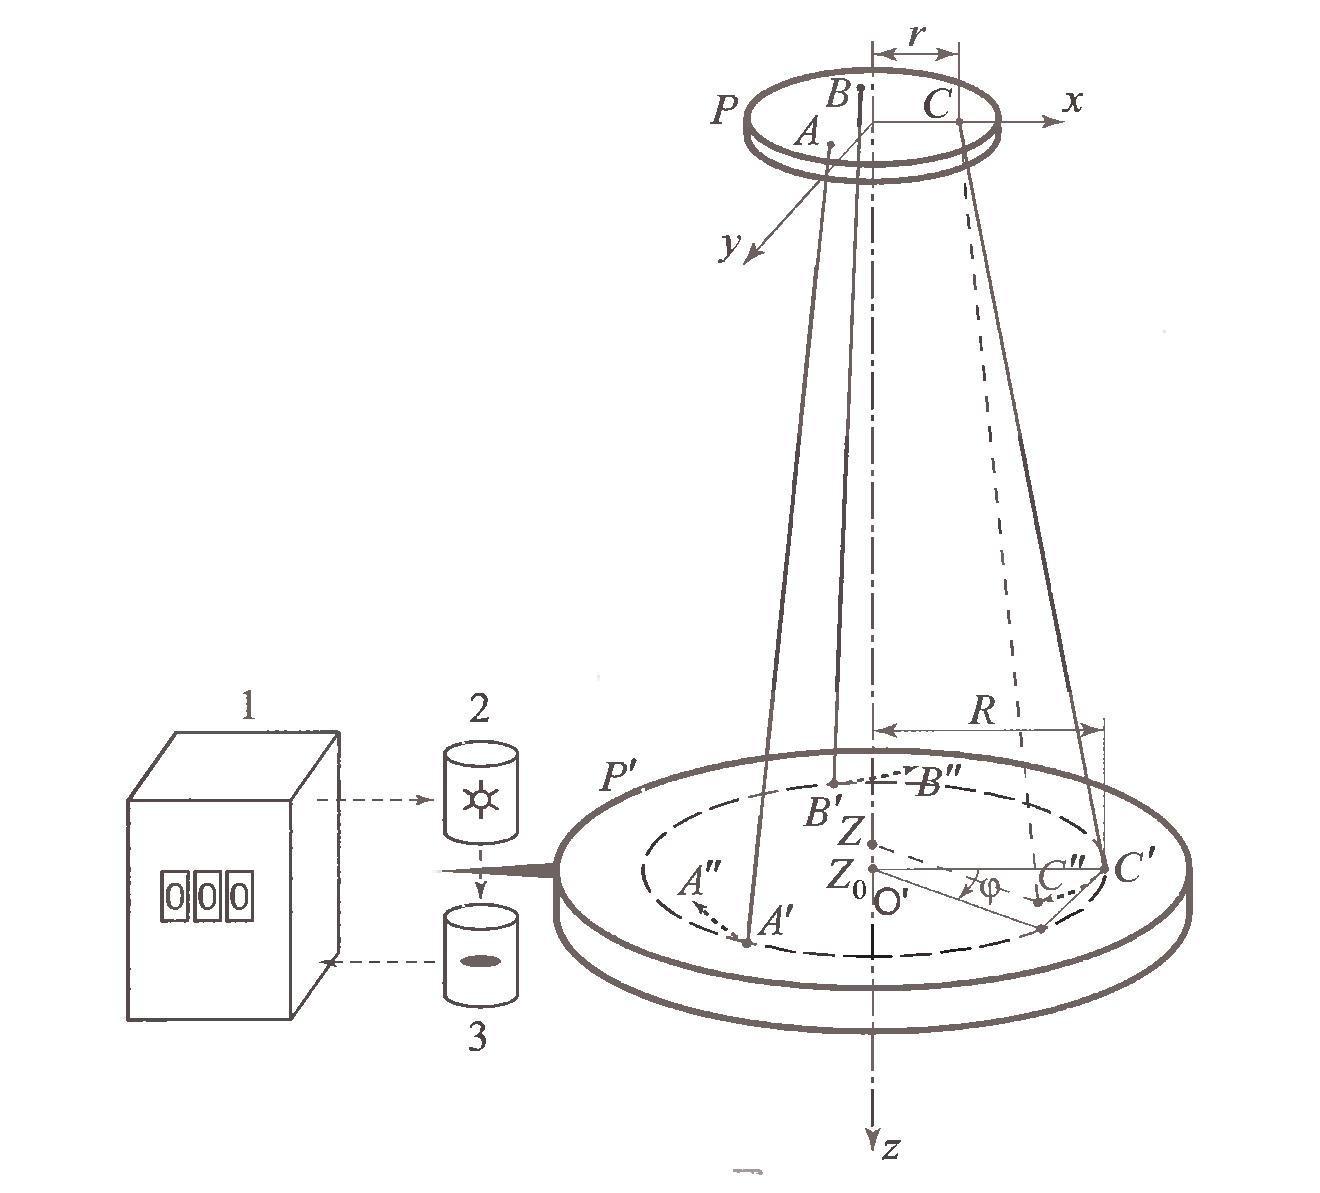
\includegraphics[scale=0.3]{schem_device}
	\caption{Трифилярный подвес}
	\label{ris1}
\end{figure}

Для однородных тел известной плотности при заданных размерах и достаточно простой форме момент инерции можно вычислить. Для неоднородных тел и тел сложной формы момент инерции можно определить экспериментально. Удобно использовать устройство, показаное на рис. \ref{ris1} и называемое трифилярным подвесом. Оно состоит из вешенной к ней на трех симметрично расположенных нитях $AA^{'}$, $BB^{'}$ и $CC^{'}$ вращающейся платформы $P^{'}$.

Платформа $P$ укреплена на кронштейне и снабжена рычагом (на рисунке не показан), при помощи которого в системе можно создать крутильные колебания путем небольшого поворота верхней платформы.

Если пренебречь потерями энергии на трение(о воздух и в креплениях нитей), то уравнение сохранения энергии при колебаниях можно записать следующим образом:
\[ \frac{I \dot{\varphi^2}}{2} + mg(z_0 - z) = E\]

Здесь $I$ -- момент инерции платформы вместе с исследуемым телом, $m$ -- масса платформы с телом, $\varphi$ -- угол повороты платформы от положения равновесия системы, точкой обозначена производная по времени (угловая скорость), $z_0$ -- координата по вертикали центра нижней платформы $O^{'}$ при равновесии ($\varphi = 0$), $z$ -- координата той же точки при некотором угле поворота $\varphi$. Первый член в левой части уравнения -- кинетическая энергия вращения, второй член -- потенциальная энергия в поле тяжести, $E$ -- полная энергия системы (платформы с тулом).

Воспользуемся системой координат $x,y,z$ связанной с верхней платформой, как показано на рис. 1. Координаты верхнего конца одной из нитей подвеса точки $C$ в 
этой системе -- $(r, 0, 0)$. Нижний конец данной нити $c^{'}$, находящейся на нижней платформе, при равновесии иметт координаты ($R,0,z_0$), а при повороте платформы на угол $\varphi$ эта точка переходит в $C^{''}$ с координатами ($R \cos{\varphi}, R\sin{\varphi},z$). Расстояние между точками $C^{'}$ и $C^{''}$ равно длине нити $L$. Поэтому 
\[ (R\cos{\varphi} - r)^2 +R^2\sin^2{\varphi} +z^2 = L^2 .\]

Учитывая, что при малых углах поворота $\cos{\varphi} \approx 1 -\dfrac{\varphi^2}{2}$, получаем 
\[ z^2 = L^2 - R^2 - r^2 +2Rr\cos{\varphi} = z_0^2 - 2Rr(1 - \cos{\varphi})\approx z_0^2 - Rr\varphi^2 .\]

Извлекая из выражения выше квадратный корень и учитывая малость угла $\varphi$, имеем 
\[ z \approx \sqrt{z_0^2 - Rr\varphi^2}\approx \sqrt{1-\frac{Rr\varphi^2}{z_0^2}}\approx z_0 = \frac{Rr-\varphi^2}{2z_0} .\]

Подставляя это значение $z$ в уравнение сохранения энергии получаем 
\[ \frac{1}{2}I \ddot{\varphi} + mg\frac{Rr}{z_0}\varphi = 0.\] 

Производная по времени от $E$ равна нулю, так как потерями энергии на трение, как уже был сказано выше, пренебрегаем.

Решение этого уравнения имеет вид 
\[ \varphi = \varphi_0\sin{\sqrt{\frac{mgRr}{Iz_0}}t + \theta} .\]

Здесь амплитуда $\varphi_0$ и физа $\theta$ колебаний определяются начальными условиями. Период крутильных колебаний нашей системы равен 
\[ T = 2\pi \sqrt{\frac{Iz_0}{mgRr}}.\]

Обратим внимание на то, что из этой формулы при $r = R$ и $I = mR^2$ (тонкое кольцо) получаем формулу для математического маятника. Из последнего уравнения находим формулу для определения момента инерции:
\[ I = \frac{mgRrT^2}{4\pi^2 z_0}.\]

Учитывая, что параметры установки $R,r$ и $z_0$ при проведении опытов не меняются, удобно переписать последнее уравнение следующим образом: 
$$\label{eq1}
I = kmT^2
$$

Здесь $k = \dfrac{gRr}{4\pi^2 z_0}$ -- величина, постоянная для данной установки.

Таким образом, полученные формулы позволяют определить момент инерции платформы с телом и отдельно платформы по соответствующим периодам крутильных колебаний.

При выводе формул предполагалось, что малы необратимые потери энергии, связанные с трением, то есть мало затухание колебаний. О затухании колебаний можно судить, сравнивая время $\tau$ уменьшения амплитуда колебаний в 2-3 раза с периодом колебаний $T$. Необратимыми потерями энергии можно пренебречь, если выполняется условие 
\[ \tau \gg T .\]

\subsection*{Ход работы}
Сперва определим погрешности приборов:
\begin{itemize}
	\item линейка: $2\cdot\dfrac{\text{цена деления}}{2} = 1$ мм
	\item секундомер: из описания прибора $0.03$ с
	\item штангенциркуль: $2\cdot\dfrac{\text{цена деления}}{2} = 0.1$ мм
\end{itemize}
\begin{enumerate}
	\item 
	Проверим, пригодна ли установка для измерений, то есть нормально ли функционирует устройство для возбуждения крутильных колебаний, не возникают ли при этом нежелательные маятниковообразные движения, работает ли счетчик числа колебаний.

	Для этого измерим время $20$ колебаний и рассчитаем период одного колебаний по формуле $T = \dfrac{t}{N}$ два раза, а затем сравним. 
	\begin{table}[h]
		\centering
		\begin{tabular}{|c|c|c|c|} \hline 
			№ опыта & Число колебаний & $t$, с 	 & $T$, с  \\ \hline 
			$1$ 	& $20$ 			  & $88.184$ & $4.409$ \\ \hline 
			$2$ 	& $20$ 			  & $88.122$ & $4.406$ \\ \hline 
		\end{tabular} 
	\end{table}

	Периоды в обоих случаях получислись практически одинаковыми. Следовательно, устройство для возбуждения крутильных колебаний функционирует нормально, нежелательных маятниковообразных движений не возникает, счетчик числа колебаний работает нормально.
	Случайная погрешность при этом равна $\sigma_T^{text{случ}} = 0.002$ c. Полная погрешность --- $\sigma_T = 0.003$ с.

	\item

	Сравним время $\tau$ уменьшения амплитуды колебаний в $2-3$ раза с периодом колебаний $T$.

	Отклоним маятник на $35^{\circ}$. Через время $t = 220.5$ секунд ($50$ колебаний) амплитуда равна $20^{\circ}$. Таким образом, $\tau \gg T$.
	
	\item 
	Найдем рабочий диапазон амплитуд колебаний.
	\begin{table}[h]
		\centering
		\begin{tabular}{|c|c|c|c|c|} \hline 
			№ опыта & $A$, $^{\circ}$ & Число колебаний & $t$, с 	 & $T$, с  \\ \hline 
			$1$ 	& $10^{\circ}$	  & $20$ 			& $87.614$ 	 & $4.381$ \\ \hline 
			$2$ 	& $20^{\circ}$	  & $20$ 			& $87.825$ 	 & $4.391$ \\ \hline 
			$3$ 	& $30^{\circ}$	  & $20$ 			& $88.401$ 	 & $4.420$ \\ \hline 
		\end{tabular} 
	\end{table}

	При амплитуде $A = 30^{\circ}$ период начинает зависеть от амплитуды. Таким образом, рабочий диапазон --- $10^{\circ} - 20^{\circ}$.

	\item Измеряем параметры установки $z_0, R, r$ (см. рис. \ref{ris1}).
	$$
	z_0 = 2.150 \pm 0.002~\text{м}
	$$
	Величина $z_0$ была определена с помощью обычной линейки, а также с помощью лазерного дальномера. Дальномер не дал хорошего результата из-за сложности в приведении маятника в равновесие.
	$$
	m = 1066.8 \pm 0.5~\text{г}
	$$
	$$
	R = 114.6 \pm 0.5~\text{мм}
	$$
	$$
	r = 30.2 \pm 0.3~\text{мм}
	$$
	По этим данным вычислим константу $k$ и ее погрешность $\sigma_k$:
	$$
	\Rightarrow~k = \frac{gRr}{4\pi^2 z_0} = 3.97\cdot 10^{-4}
	$$ 
	\begin{multline*}
		\sigma_k = \sqrt{\left(\frac{\partial{k}}{\partial{R}}\right)^2\cdot\sigma_R^2 + \left(\frac{\partial{k}}{\partial{r}}\right)^2\cdot \sigma_r^2 + \left(\frac{\partial{k}}{\partial{z_0}}\right)^2\cdot \sigma_{z_0}^2} =  \\
		= \sqrt{\left(\frac{gr}{4\pi^2z_0}\right)^2\cdot \sigma_R^2 + \left(\frac{gR}{4\pi^2z_0}\right)^2\cdot \sigma_r^2 +  \left(\frac{gRr}{4\pi^2 z_0^2}\right)^2\cdot \sigma_{z_0}^2} = 4.36\cdot10^{-6}
	\end{multline*}
	Итоговое значение для $k$:
	$$
	k = (3.97 \pm 0.04)\cdot 10^{-4}
	$$

	\item Определим момент инерции ненагруженной платформы (здесь и далее периоды колебаний будем определять с относительной погрешностью не хуже $0.5\%$).
	
	Для определения момента инерции установки возбудим крутильные колебания ненагруженной платформы. Измерим период колебаний ненагруженной платформы. Для этого измерим время $N$ полных колебаний установки. По результатам измерений определим $ T_{0} = \dfrac{t}{N}$. В пункте 1 мы получили $T = 4.408 \pm 0.002$ c. Тогда рассчитаем момент инерции ненагруженной платформы по формуле (\ref{eq1}).
	$$
	I_0 = kmT^2 = 8.23\cdot 10^{-3}~\text{кг$\cdot$м$^2$}
	$$
	Погрешность $I_0$ найдем по формуле
	\begin{multline*}
	\sigma_{I_0} = \sqrt{\left(\frac{\partial{I_0}}{\partial{k}}\right)^2\cdot\sigma_k^2 + \left(\frac{\partial{I_0}}{\partial{m}}\right)^2\cdot \sigma_m^2 + \left(\frac{\partial{I_0}}{\partial{T}}\right)^2\cdot \sigma_T^2} =  \\
		= \sqrt{\left(mT^2\right)^2\cdot \sigma_k^2 + \left(kT^2\right)^2\cdot \sigma_m^2 +  \left(2kmT\right)^2\cdot \sigma_T^2} = 8.33\cdot 10^{-5}
	\end{multline*}
	Итоговое значение $I_0$:
	$$
	I_0 = (8.23\pm 0.08)\cdot 10^{-3}~\text{кг$\cdot$м$^2$}
	$$

	\item
	Измеряем моменты инерции различных тел из имеющегося набора. Сначала порознь, а затем вместе. Помещать тела на платформу будем там, чтобы общий центр масс всегда находился на оси вращения (оси симметрии) системы, то есть чтобы не было заметного перекоса платформы. По полученным данным проверяем аддитивность моментов инерции, то есть справедливость соотношения $I = I_1 + I_2$, где $I_1$ и $I_2$ --- моменты инерции первого и второго тел, а $I$ --- общий момент инерции. Погрешность, с которой выполняется это соотношение, является хорошей мерой точности проводимых измерений. Так же рассчитаем теоретически моменты инерции $I$ всех используемых в эксперименте тел и сравним результаты с измеренными экспериментально значениями $I$.
	\begin{table}[ht!]
		\centering
		\begin{tabular}{|l|c|c|c|c|c|}
			\hline
			Тело & $n$ & $t$, с & $T$, с & $\overline{T}$, с & $m$, г \\ \hline
			\multirow{2}{*}{платформа} & \multirow{2}{*}{$20$} & $88.184$ & $4.409$ & \multirow{2}{*}{$4.408$} & \multirow{2}{*}{$1066.8$} \\
			 & & $88.122$ & $4.406$ & \\ \hline
			\multirow{2}{*}{платформа, кольцо} & \multirow{2}{*}{$20$} & $83.857$ & $4.193$ & \multirow{2}{*}{$4.188$} & \multirow{2}{*}{$1844.3$} \\
			 & & $83.652$ & $4.183$ & \\ \hline
			\multirow{2}{*}{платформа, диск} & \multirow{2}{*}{$20$} & $78.561$ & $3.928$ & \multirow{2}{*}{$3.927$} & \multirow{2}{*}{$1657.1$} \\
			 & & $78.500$ & $3.925$ & \\ \hline
			\multirow{2}{*}{платформа, кольцо, диск} & \multirow{2}{*}{$20$} & $79.071$ & $3.954$ & \multirow{2}{*}{$3.950$} & \multirow{2}{*}{$2434.6$} \\
			 & & $78.925$ & $3.946$ & \\ \hline
		\end{tabular}
		\caption{Периоды колебаний для различных тел на трифилярном подвесе.}
		\label{tab:periods_diff_body}
	\end{table}

	Запишем в таблицу \ref{tab:moments} рассчитанные теоретически и экспериментально моменты инерции.
	
	Экспериментальные моменты инерции вычисляем по формуле
	$$
	I = kmT^2
	$$
	Погрешности по формуле
	$$
	\sigma_{I_0} = \sqrt{\left(\frac{\partial{I_0}}{\partial{k}}\right)^2\cdot\sigma_k^2 + \left(\frac{\partial{I_0}}{\partial{m}}\right)^2\cdot \sigma_m^2 + \left(\frac{\partial{I_0}}{\partial{T}}\right)^2\cdot \sigma_T^2}
	$$
	\begin{table}[h!]
		\centering
		\begin{tabular}{|l|c|r|}
			\hline
			Тело & $I_{theor}$, кг$\cdot$м$^{2}$, $10^{-3}$ & $I_{exp}$, кг$\cdot$м$^{2}$, $10^{-3}$ \\ \hline
			Платформа & $8.27$ & $8.23\pm 0.08$ \\ \hline
			Платформа + кольцо & $12.91$ & $12.84\pm 0.13$ \\ \hline
			Кольцо & $4.64$ & $4.61\pm 0.15$ \\ \hline
			Платформа + диск & $10.20$ & $10.15\pm 0.10$ \\ \hline
			Диск & $1.93$ & $1.92\pm 0.13$ \\ \hline
			Платформа + диск + кольцо & $14.84$ & $15.08\pm 0.15$ \\ \hline
			Диск + кольцо & $6.57$ & $6.85\pm 0.17$ \\ \hline
		\end{tabular}
		\caption{Моменты инерции различных тел}
		\label{tab:moments}				
	\end{table}

	Для расчетов теоретических значений использованы следующие харктеристики тел:
	\begin{itemize}
		\item \textit{Платформа}

		Диаметр платформы: $D = 24.5\pm 0.1$ см

		Масса платформы: $m = 1066.8\pm 0.5$ г

		Платформа представляет собой однородный цилиндр. Момент инерции: $$I = \dfrac{1}{2}mR^2$$
		
		\item \textit{Кольцо}

		Внешний диаметр кольца: $D_1 = 15.89\pm 0.01$ см

		Толщина кольца: $r = 4.1$ мм 

		Внутренний диаметр кольца: $D_2 = D_1 - 2r = 15.07\pm0.01$ см

		Масса кольца: $m = 777.5\pm 0.5$ г

		Кольцо представляет собой толстостенный полый цилиндр. Момент инерции: $$I = \dfrac{1}{2}m(R_1^2+R_2^2)$$ 

		\item \textit{Диск}
		
		Диаметр диска: $D = 16.15\pm 0.01$ см

		Высота диска: $H = 3.6\pm 0.1$ мм

		На диске имеется выступ, представляющий собой сплошной цилиндр. Диаметр: $d = 1.04\pm 0.01$ см, высота: $h = 2.52\pm 0.01$ см. Определим массу выступа $m_1$ и массу диска $m_2$. Полная масса $m = 590.3\pm 0.5$ г.
		$$
		m = m_1 + m_2
		$$
		$$
		\frac{m_2}{m_1} = \frac{\rho\cdot\pi R^2H}{\rho\cdot\pi r^2h} = \frac{HR^2}{hr^2} = 122.5
		$$
		$$
		m = m_1 + 122.5m_1~\Rightarrow~m_1 = 4.8\pm 0.5~\text{г},~m_2 = 585.5\pm 0.5~\text{г}
		$$
		Момент инерции и диска, и выступа находятся по формуле $I = \dfrac{1}{2}mR^2$. Полный момент инерции тела находится как сумма моментов инерции его частей.
	\end{itemize}
	Мы видим, что рассчитанные теоретически значения близки к полученным экспериментально. Следовательно, момент инерции тела --- аддитивная величина.

	\item
	Определим зависимость момента инерции системы тел от их взаимного расположения. Поместим на платформу диск, разрезанный по диаметру. Постепенно раздвигая половинки диска так, чтобы их общий центр масс все время оставался на оси вращения платфомры, снимаем зависимость момента инерции такой системы $I$ от расстояния $h$ каждой из половинок до оси вращения (центра платформы).
	
	Суммарная масса половинок диска --- $m = 1131.6\pm 0.5$ г.
	
	Полученные данные запишем в таблицу \ref{tab:position}.
	\begin{table}[h!]
		\centering
		\begin{tabular}{|c|c|c|c|c|c|} \hline
			№ опыта 			  & $h$, см 				 & $t$, c 	& $T$, c  & $\overline{T}$, c 		 & $I$, $10^{-3}$ кг$\cdot$м$^2$ \\ \hline
			\multirow{2}{*}{$1$}  & \multirow{2}{*}{$0$} 	 & $65.375$ & $3.269$ & \multirow{2}{*}{$3.265$} & \multirow{2}{*}{$9.30$} 		 \\ 
								  & 	    			 	 & $65.191$ & $3.260$ & 						 \\ \hline
			\multirow{2}{*}{$2$}  & \multirow{2}{*}{$7.85$}  & $85.951$ & $4.298$ & \multirow{2}{*}{$4.295$} & \multirow{2}{*}{$16.10$}		 \\ 
			 	    			  &						 	 & $85.832$ & $4.292$ & 						 \\ \hline
			\multirow{2}{*}{$3$}  & \multirow{2}{*}{$6.85$}  & $81.598$ & $4.080$ & \multirow{2}{*}{$4.086$} & \multirow{2}{*}{$14.57$}		 \\ 
			 	    			  &						 	 & $81.812$ & $4.091$ & 						 \\ \hline
			\multirow{2}{*}{$4$}  & \multirow{2}{*}{$5.85$}  & $77.271$ & $3.864$ & \multirow{2}{*}{$3.862$} & \multirow{2}{*}{$13.02$} 	 \\ 
								  &						 	 & $77.202$ & $3.860$ & 						 \\ \hline
			\multirow{2}{*}{$5$}  & \multirow{2}{*}{$4.85$}  & $73.598$ & $3.680$ & \multirow{2}{*}{$3.682$} & \multirow{2}{*}{$11.83$}		 \\ 
								  &						 	 & $73.674$ & $3.684$ & 						 \\ \hline
			\multirow{2}{*}{$6$}  & \multirow{2}{*}{$3.85$}  & $70.758$ & $3.538$ & \multirow{2}{*}{$3.542$} & \multirow{2}{*}{$10.95$}		 \\ 
								  &						 	 & $70.912$ & $3.546$ & 						 \\ \hline
			\multirow{2}{*}{$7$}  & \multirow{2}{*}{$2.85$}  & $67.902$ & $3.395$ & \multirow{2}{*}{$3.392$} & \multirow{2}{*}{$10.04$}		 \\ 
								  &						 	 & $67.759$ & $3.388$ & 						 \\ \hline
			\multirow{2}{*}{$8$}  & \multirow{2}{*}{$1.85$}  & $66.423$ & $3.321$ & \multirow{2}{*}{$3.318$} & \multirow{2}{*}{$9.61$}		 \\ 
								  &						 	 & $66.306$ & $3.315$ & 						 \\ \hline
			\multirow{2}{*}{$9$}  & \multirow{2}{*}{$0.85$}  & $65.262$ & $3.263$ & \multirow{2}{*}{$3.269$} & \multirow{2}{*}{$9.33$}		 \\ 
								  &						 	 & $65.482$ & $3.274$ & 						 \\ \hline
		\end{tabular}
		\caption{Моменты инерции различных тел}
		\label{tab:position}				
	\end{table}

	Построим график полученной зависимость $I(h^2)$ и определим по нему массу и момент инерции диска: зависимость имеет вид $y = kx + b$, где $y = I$, $x = h^2$. Тогда $k$ --- масса половинок диска, $b$ --- момент инерции платформы с диском в центре.
	\begin{figure}[h]
		\centering
		\begin{tikzpicture}[dot/.style = {draw, fill = black, color = black, circle, inner sep=1.5pt}, >=stealth]
			\begin{axis}
				[
				width = 0.7\paperwidth, 
				xlabel = {$h^2$, см$^2$}, 
				ylabel = {$I$, $10^{-3}$ кг$\cdot$м$^2$}, 
				grid=both, 
				ymin = 8, ymax = 17,
				xmin = 0, xmax = 70,
				]
				
				\addplot+[black,only marks,mark = *,
				mark options = {
					scale = 1.0, 
					fill = black
				}] coordinates {(0, 9.3) (0.7225, 9.33) (3.4225, 9.61) (8.1225, 10.04) (14.8225, 10.95) (23.5225, 11.83) (34.2225, 13.02) (46.9225, 14.57) (61.6225, 16.10)};
				\addplot[black, domain=0:65] {9.23595 + 0.1118 * x};
			\end{axis}
		\end{tikzpicture}
	\end{figure}

	Пользуюясь методом наименьших квадратов найдем коэффициент наклона графика по формуле:
	\[k = \frac{<x y> - <x> <y>}{<x^2> - {<x>}^2}  = 0.11035~\frac{\text{$10^{-3}$ кг$\cdot$м$^2$}}{\text{см$^2$}}\]
	Тогда масса диска равна
	$$
	m = 1103.5~\text{г}
	$$
	Найдем случайную погрешность углового коэффициента по формуле :
	\[{\sigma_k}^{\text{сл}}= \sqrt{\frac{1}{n-2}\left(\frac{D_{yy}}{D_{xx}} - k^2 \right)} = 6.9~\text{г}\]
	Таким образом,
	$$
	m = 1.1035\pm 0.0069~\text{кг}
	$$
	Полученное значение хорошо согласуется с реальной массой диска. Момент инерции платформы с диском в центре также совпадает с настоящим.
	\newpage
	\textbf{Вывод}

	\begin{itemize}
		\item Величина момента инерции, определенная с помощью трифилярного подвеса с довольно большой точностью совпадает с теоретическими предсказаниями. Большая точность обеспечивается малой погрешностью измерения времени, а также выбором условий, при которых крутильные колебания подвеса можно считать слабозатухающими.
		\item Была достигнута относительная точность определения момента инерции $ \varepsilon_{I}\approx 1\% $. Основной вклад в погрешность измерения момента инерции внесла погрешность косвенного измерения $z_{0}$. Данную погрешность можно уменьшить, если более точно определить параметры установки.
		\item Была полученая зависимость $ I(h^{2}) $. Данная зависимость довольно хорошо аппроксимируется линейной зависимость, что подтверждает теоретические данные.
		\item Была подтверждена аддитивность момента инерции.
	\end{itemize}
\end{enumerate}

\end{document}